\documentclass[a4paper,12pt]{article}
\usepackage[hmargin=2cm,top=4cm,headheight=65pt,footskip=45pt]{geometry}
\usepackage[utf8]{inputenc}
\usepackage{graphicx}
\usepackage[hidelinks]{hyperref}
\usepackage{array}
\usepackage{lastpage}
\usepackage{lipsum}
\usepackage{fancyvrb}
\usepackage{color}
\usepackage{fancyhdr}
\usepackage{amsmath}
\usepackage{enumitem}
\usepackage{titlesec}
\usepackage{floatrow}
\newfloatcommand{capbtabbox}{table}[][\FBwidth]

\definecolor{customGray}{RGB}{128,128,128}
%\definecolor{Eblue}{RGB}{0,21,87}
%\definecolor{Eblue}{rgb}{0.2, 0.2, 0.6}
\definecolor{Eblue}{rgb}{0.0, 0.18, 0.39}
%==============Header & Footnote==============

\pagestyle{fancy}
\renewcommand{\headrulewidth}{0pt}
\fancyhead[C,CO,L,LO,R,RO]{}
\fancyhead[C]{%
          \begin{tabular}{|m{3.0cm}|m{10.0cm}|m{2.5cm}|}
          \hline
          \centering\vspace{1.75mm}
\includegraphics[scale=0.275]{logo.pdf} &
          \centering
          {\footnotesize {\sf UNIVERSIDAD EAFIT\\ SCHOOL OF ENGINEERING\\
          \vspace{-1mm}DEPARTMENT OF SYSTEMS AND INFORMATICS}} &
          \centering
          \footnotesize{Page \thepage\ de \pageref{LastPage}\\
          ST245\\
          \vspace{-0.75mm}Data Structures
          }\tabularnewline
          \hline
          \end{tabular}
}
\fancyfoot[C,CO,L,LO,R,RO]{}
\fancyfoot[C]{
          \begin{centering}
            \textcolor{customGray}{{\footnotesize {\sf Professor Mauricio Toro Bermúdez\\
            Phone: $(+57) (4) 261 95 00$ Ext. $9473$. Office: $19 - 627$\\
            \vspace{-1mm}E-mail: mtorobe@eafit.edu.co}}}
        \end{centering}
}

%=============CustomEnumItem===========

\setlist[enumerate]{label=\color{Eblue}\textbf{\roman*.}}

%=============CustomSecSubSec==========

\titleformat{\section}[hang]
{\normalsize\bfseries\itshape\color{black}}{\bfseries\itshape\color{Eblue}\thesection)}{2.5mm}{}

\titleformat{\subsection}[hang]
{\normalsize\bfseries\itshape\color{black}}{\bfseries\color{Eblue}\thesection.\alph{subsection}.}{2.5mm}{}

%==============Title==============

\title{\color{Eblue}\textbf{Laboratory practice No. 2: Big O Notation}}
\author{
  \textbf{Juan S. Cárdenas Rodríguez}\\
  Universidad EAFIT\\
  Medellín, Colombia\\
  jscardenar@eafit.edu.co
\and
  \textbf{David Plazas Escudero}\\
  Universidad EAFIT\\
  Medellín, Colombia\\
  dplazas@eafit.edu.co
}

%=============Document=============
\begin{document}
  \maketitle
  \thispagestyle{fancy}

  \section{ONLINE EXERCISES (CODINGBAT)}
  \subsection{Array II}
    \begin{enumerate}
      \item \begin{Verbatim}
        public int[] zeroFront(int[] nums) {             // c0
            boolean [] used = new boolean [nums.length]; // c1
            int cont = 0;                                // c2
            for (int i = 0; i < nums.length; i++) {      // c3 + n
              if(nums[i] == 0) {                         // c4 + n
                if (i != cont) {                         // c5 + n
                  nums[i] = nums[cont];                  // c6 + n
                  nums[cont] = 0;                        // c7 + n
                }
                cont++;                                  // c8 + n
              }
            }
            return nums;                                 // c9
          }
      \end{Verbatim}
      Therefore, \texttt{zeroFront} is $O(c_0+c_1+c_2+c_3+c_4+c_5+c_6+c_7+c_8+c_9+6n)$.
      Applying the sum and product properties, \texttt{zeroFont} is $O(n)$.

      \item \begin{Verbatim}
      public int[] notAlone(int[] nums, int val) {       // c0
          for(int i = 1; i < nums.length-1; i++) {       // c1 + n
            if(nums[i] == val && nums[i-1] != val
              && nums[i+1] != val) {                     // c2 + n
              if (nums[i-1] > nums[i+1])                 // c3 + n
                nums[i] = nums[i-1];                     // c4 + n
              else                                       // c5 + n
                nums[i] = nums[i+1];                     // c6 + n
            }
          }
          return nums;                                   // c7
        }
    \end{Verbatim}
    Therefore, \texttt{notAlone} is $O(c_1+c_2+c_3+c_4+c_5+c_6+c_7+6n)$.
    Applying the sum and product properties, \texttt{notAlone} is $O(n)$.

    \item \begin{Verbatim}
    public boolean tripleUp(int[] nums) {                // c0
      for (int i = 0; i < nums.length - 2; i++) {        // c1 + n-2
        if(nums[i] + 1 == nums[i+1] && nums[i]
         + 2 == nums[i+2]) return true;                  // c2
      }
      return false;                                      // c3
    }
    \end{Verbatim}
    \texttt{tripleUp} is $O(c_0+c_1+c_2+c_3+n-2)$. When we apply the product
    and sum properties, \texttt{tripleUp} is $O(n)$.

    \item \begin{Verbatim}
    public int[] tenRun(int[] nums) {                   // c0
      int tempMult = 0;                                 // c1
      boolean used = false;                             // c2
      for(int i = 0; i < nums.length; i++) {            // c3 + n
        if (nums[i] % 10 == 0) {                        // c4 + n
          used = true;                                  // c5 + n
          tempMult = nums[i];                           // c6 + n
        }                                               // c7 + n
        if(used)                                        
          nums[i] = tempMult;
      }
      return nums;
    }
    \end{Verbatim}

    \item \begin{Verbatim}
    public int[] shiftLeft(int[] nums) {
      int [] mod = new int[nums.length];
      if (nums.length==1) return nums;
      for (int i=1; i<nums.length; i++) {
        mod[nums.length-1]=nums[0];
        mod[i-1]=nums[i];
      }
      return mod;
    }
    \end{Verbatim}
    \end{enumerate}

    \subsection{Array III}
    \begin{enumerate}
      \item \begin{Verbatim}
      public int[] seriesUp(int n) {
        int no = n*(n+1)/2;
        int [] nums = new int [no];
        int a = 0;
        for (int i = 1; i <= n; i++) {
          for (int j = 1; j <= i; j++) {
            nums[a] = j;
            a++;
          }
        }
        return nums;
      }
      \end{Verbatim}

      \item\begin{Verbatim}
      public int countClumps(int[] nums) {
        int c = 0;
        for (int i = 0; i < nums.length-1; i++) {
          if (nums[i] == nums[i+1]) {
            for (int j = i; j < nums.length; j++) {
              if (nums[j] != nums[i]) {
                i = j;
                c++;
              }
              if (c == 0 && j == nums.length-1) {
                c++;
              }
            }
          }
        }
        return c;
      }
      \end{Verbatim}

      \item \begin{Verbatim}
      public boolean linearIn(int[] outer, int[] inner) {
        int j = 0;
        int c = 0;
        if (inner.length == 0) {
          return true;
        }
        for (int i = 0; i < outer.length; i++) {
          if (inner[j] == outer[i]) {
            j++;
            if (j==inner.length) {
              return true;
            }
          }
        }
        return false;
      }
      \end{Verbatim}

      \item \begin{Verbatim}
      public int[] fix45(int[] nums) {
        boolean [] arr = new boolean[nums.length];
        for (int i = 0; i < nums.length-1; i++) {
          if (nums[i] == 4 && nums[i+1] == 5) {
            arr[i+1] = true;
          } else  if (nums[i] == 4 && nums[i+1] != 5) {
            for (int j = 0; j < nums.length; j++) {
              if (nums[j] == 5 && arr[j] == false) {
                nums[j] = nums[i+1];
                nums[i+1] = 5;
                arr[i+1] = true;
                break;
              }
            }
          }
        }
        return nums;
      }
      \end{Verbatim}
    \end{enumerate}




    \section{SIMULATION OF PROJECT PRESENTATION QUESTIONS}
    \subsection{ArrayMax}
    \begin{figure}[ht]
      \begin{floatrow}
        \ffigbox{
          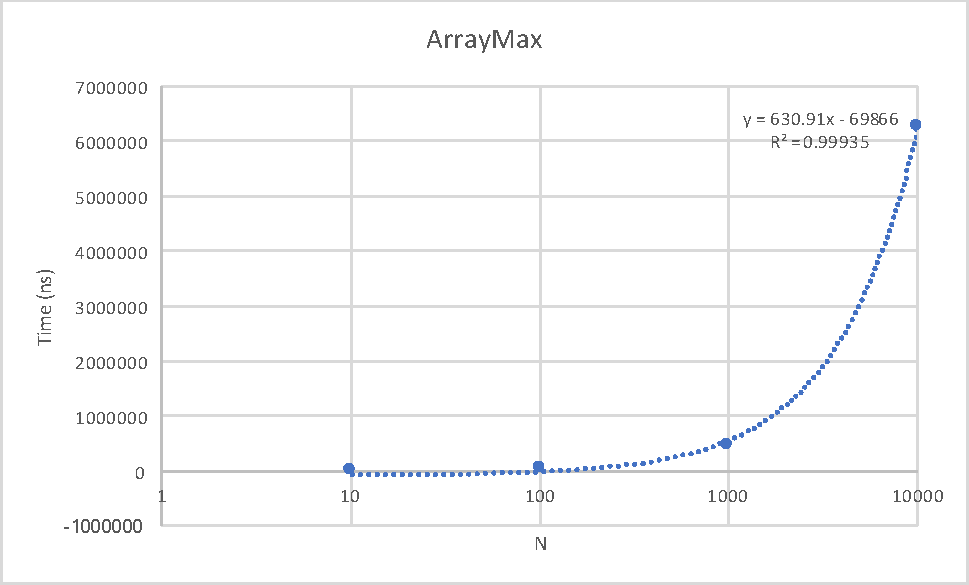
\includegraphics[scale=0.45]{ArrayMax.pdf}
        }{
          \caption{Time vs. N for ArrayMax}
        }
        \capbtabbox{
          \begin{tabular}{cc}
            \hline
            \textbf{N} & \textbf{Time (ns)} \\ \hline
            10         & 6000               \\
            100        & 27000              \\
            1000       & 346000             \\
            10000      & 6717000            \\ \hline
          \end{tabular}
        }{
          \caption{ArrayMax's data.}
        }
      \end{floatrow}
    \end{figure}

    \section{EXAM SIMULATION}
    \begin{enumerate}
      \item $\texttt{start}+1,\quad \texttt{nums},\quad \texttt{target}$
      \item a) $T(n) = T(n/2) + C$
      \item $n-a, a, b, c$\\
      res, solucionar($n-b,a,b,c$)+1\\
      res, solucionar($n-c,a,b,c$)+1
      \item e) La suma de los elementos de a y es $O(n)$.
    \end{enumerate}


    \newpage
    \bibliographystyle{plain}
    \bibliography{Lab.bib}
\end{document}
